\documentclass{article}
\usepackage[left=2cm,right=2cm,top=2cm,bottom=2cm]{geometry} 
\usepackage{blindtext}
\usepackage{graphicx} 
\usepackage[section]{placeins} 
\usepackage[spanish]{babel}
\usepackage{listings} 
\usepackage{xcolor} 
\usepackage{pdfpages}
\setcounter{secnumdepth}{2}

%------------------------------ Constants ---------------------------------
\newcommand{\nombre}{Renato Flores}
\newcommand{\carnet}{201709244}
\newcommand{\universidad}{USAC}
\newcommand{\catedratico}{Ing. Allan Morataya}
\newcommand{\curso}{Sistemas Operativos 1}
\newcommand{\titulo}{Hoja de trabajo \#1}
%----------------------- Custom commands ------------------------------
\newcommand*\rbreak{\par\noindent\linebreak}

\author{\nombre , \carnet}
\title{\textbf{\Huge\titulo}\\Reforzamiento de conceptos}

\graphicspath{{/home/renato/screenshots/renato/second-semester-2020/sopes-1/agosto-10/}}

\begin{document}
\maketitle
\section{Explique en qué consiste un sistema operativo.}
Software que controla la computadora y administra los servicios y recursos disponibles. Permite controlar las asignaciones de memoria, ordernar las solicitudes al sistema, controlar los dispositivos de entrada y salida, facilitar la conexión de redes y el manejo de archivos. 

\section{Justifique porque la arquitectura de un SO está diseñada por capas.}
Un SO se diseña en capas con el objetivo de poder abstraer la complejidad del hardware subyacente poco a poco. De esta forma, la capa mas cercana al núcleo (Controlador de interrupciones) se centra y optimiza lo mas posible para suplir esa función unicamente. Logrando que las demas capas que van encima puedan utilizar las herramientas proveídas por las capas inferiores y concentrarse en cumplir tareas cada vez de más alto nivel, ocultando en cada capa parte de la complejidad inherente a la programación en bajo nivel. El modelo de diseño en capas, además de obtener una abstracción gradual del hardware también resulta muy útil para encontrar errores, modularizar el trabajo y facilita la construcción del SO en equipos. Cada equipo asociado al desarrollo de una capa. 

\section{Defina el concepto de proceso.}
Un proceso es un programa en ejecución. Un proceso no es un programa, ya que 
el programa es un conjunto de instrucciones como tal y un proceso es cuando 
ese conjunto de instrucciones se encuentra en ejecución.
Un proceso puede levantar más subprocesos según indique el programa.
Todo proceso tiene asignado un espacio de direcciones en memoria para operar, designado por el SO.

\section{Que es la memoria MDA?}
Es un metodo denominado formalmente como Acceso Directo a la Memoria, el cual le permite a ciertos dispositivos de entrada/salida acceder directamente a la memoria principal (RAM) sin necesidad de esperar a que el CPU se desocupe para atender al dispositivo. El objetivo es aprovechar los tiempos de espera del CPU.

\section{¿En qué consiste la planificación de procesos?}
La planificación de procesos consiste en decidir que procesos se atienden en que momento, ya que la mayoría del tiempo hay varios procesos en estado ready que pueden ser puestos en ejecución, pero solo uno a la vez puede ser ejecutado por el CPU. El encargado de tomar la decisión de cuando se atiende a cada proceso se le denomina Scheduler. El algoritmo en el que Scheduler se basa para tomar la decisión varía de acuerdo a la implementación. Algunas de las preguntas clave que se hace el Scheduler antes de tomar una decisión son:
\begin{itemize}
	\item ejecutar el padre o el hijo?
	\item Proceso bloquea por semáforo: que hacer? 
	\item Proceso bloquea por I/O listo: entrar el proceso que paso de bloqueado a listo? 
	\item  Entrar al proceso interrumpido? 
\end{itemize}
\section{¿En qué consiste un sistema operativo online?}
Un sistema operativo online es una interface de usuario (UI) que habilita a los usuarios a accesar aplicaciones almacenadas completamente o parcialmente en la nube. Generalmente imitan la interfaz de un sitema opeartivo tradicional como Windows, sin embargo no son Sistemas Operativos reales en el sentido estricto de la palabra, ya que no manejan ningun tipo de hardware directamente.

\section{Mencione y explique dos estados de un proceso.}
	\subsection{Listo}
		Un usuario listo es un proceso recien creado que ha sido registrado por el Scheduler como un proceso valido para comenzar su ejecución.
	\subsection{Terminado}
		Un proceso que ha terminado su ejecución. El SO procede a liberar su espacio en memoria para dar lugar a otros procesos. Un proceso puede terminar voluntariamente o involuntariamente.
			
\section{¿Cuál es la diferencia entre aborto y suspensión, en relación a los procesos de un SO?}
	El \textbf{aborto} de un proceso fuerza el fin de su ejecución. Enviando el proceso del estado en ejecución al estado finalizado. Esto implica que toda la información que el proceso estaba utilizando en su espacio de memoria es desocupado y puede ser utilizado por otro proceso.\\
	La \textbf{suspensión} de un proceso no fuerza la terminación de su ejecución, sino simplemente se deja en un estado de espera. Su espacio en memoria se mantiene reservado, pero el CPU se libera y puede atender otro proceso mientras el proceso en cuestión se encuentra en suspesión. Posteriormente el proceso puede ser reanudado y continuar su ejecución o puede ser abortado. El SO sabe cuando la memoria RAM esta llena y si existen procesos en suspensión. De ser así, generalmente los datos del espacio de memoria de dichos procesos se mueven al Swap para dar lugar en la RAM a nuevos procesos.
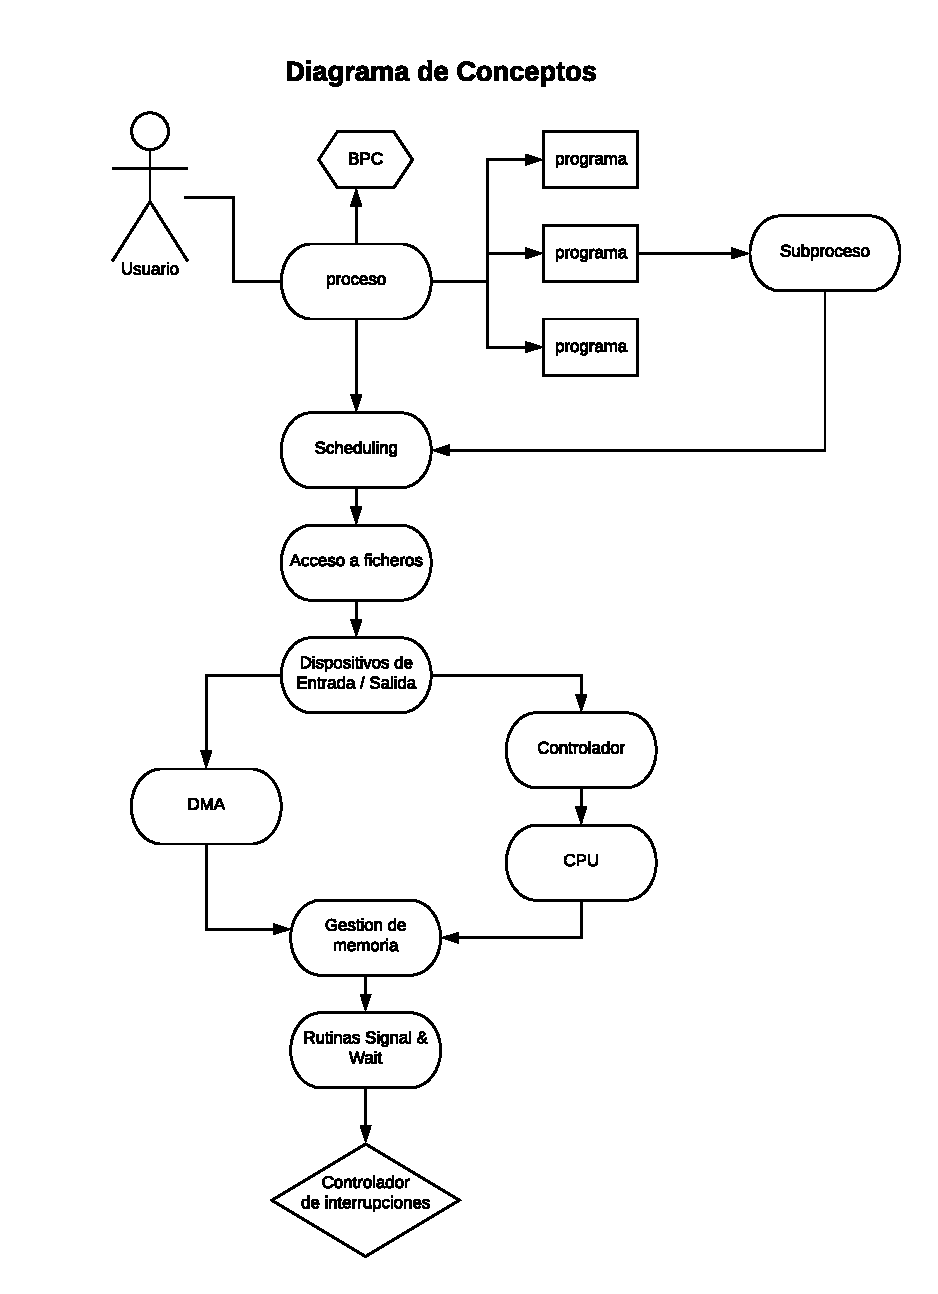
\includepdf{/home/renato/latex/general/diagram.pdf}	
	
\end{document}
